% final.tex
% Final Report for NM5660 Independent Study Module
% Author: Yih-Lun Huang
% Revisions: 16 April 2010

\documentclass{acm_proc_article-sp}

\usepackage{verbatim}

\begin{document}

\title{Investigation of the relationship between transparency and user
  experience}

\numberofauthors{1}
\author{
\alignauthor Yih-Lun Huang\\
\affaddr{HY090191Y}\\
\email{ylhuang@nus.edu.sg}
}

\maketitle
\begin{abstract}
FIXME.
\end{abstract}

\category{H.5.2}{Information Interfaces And Presentation}{User
  Interface}[input devices and strategies]

\terms{Design, Algorithms, Measurement}

\keywords{Input device, multi-touch, touchpad, lazy}

\section{Introduction}
When junior software engineers are given the task of designing a new
product or system\footnote{In the following text, ``product'' or
  ``system'' is used as a general term to refer to a product, system,
  service, or non-commercial item.}, most of the time, they tend to
squeeze as many features as possible into whatever they are suppose to
design. The interfaces between the user and the design are scattered
all over. This can often be observed in corporates where a junior
software engineer is assigned to develop an internal tool to
facilitate an existing working process (Figure~\ref{fig:featureful}.)
Though the design is practical, it is not very useful and the usage is
limited to only a small selected group of users.

\begin{figure}[!t]
\centering
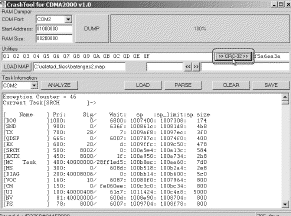
\includegraphics[width=.7\columnwidth]{featureful}
\caption{Internal tool for parsing the content in RAM.}
\label{fig:featureful}
\end{figure}

Software engineers have weird sense of excitement when they acquire
new technologies and are often very eager to try them out. Lack of
proper testing platform, many software engineers simply test the newly
acquired technology on whatever task they have at hand. Since efforts
and time are already spent on making the new technology functional and
it also provides a ``cool'' new feature to the original product, the
test is not removed afterward but instead becomes part of the product.

This is indicated by Alan Cooper that although software engineers work
hard to make their software easy to use, their frame of reference is
themselves and as a result they make it easy for other software
engineers, instead of normal users. He explains that since having too
much influence over the design of the human interface and the lack of
skills in this area, software engineers do a poor job of it
\cite{inmates:cooper}.

% TODO: talk about user-centered design and usability
This phenomenon will last until the software engineers are introduced
to the concept of usability. Dated back since the 1980s, this concept
was introduced by the published studies and analysis papers from a
dedicated group of mostly psychologists and human factors researchers
\cite{human:rubinstein, friendly:simpson, human:shneiderman,
  human:brown, software:dumas}. The philosophy behind this is that
every stage of the development process---requirements, design,
implementation, verification, and maintenance---are given great
attention to the needs and limitations of the users.

In this user-oriented development, contrast to the previous
technology-oriented or feature-oriented development, software
engineers work with experts from various specific fields---and most
importantly, also collaborate closely with the actual users---to bring
efficient, easy-to-learn, easy-to-memorize, and non-disruptive product
to the user. They form psychology and physiology model of the user to
anticipate their needs and limitations. And from that model, the
software engineers can build the product that would perfectly fit the
users.

% Bring up transparency, disrupt
From their field research, Holtzblatt et al.\ show that elements of an
application design can disrupt users' work. They observed that only
when the users are not disrupted by the computer system will they
remain in the flow of their work and experience interface transparency
\cite{transparency:holtzblatt}. This interface transparency is the
ultimate goal for usability studies and is considered as the ideal
relationship between user and tool with the tool seeming to disappear
by Rutkoski \cite{transparency:rutkoski}.

% danger of transparency
However, the idea of striving for interface transparency is also
challenged by others. Bolter and Gromala talked about the myth of
transparency:
\begin{quote}
\textit{The danger of transparency is that the interface will mask the
operation of the system exactly when the user needs to see and
understand what the system is doing.} \cite{windows:bolter}.
\end{quote}
As described by Norman, the designers and the users each have their
own conceptual models or mental images of the product. Ideally, these
two models should be identical for the users to understand and use the
product properly. Unfortunately, this might not always be the case. So
the users often have to form their own model exclusively from the
observation of the product, whether from the exterior guise, the
feedback provided, the responses from blogger, documentations, and etc
\cite{design:norman}. Therefore, if the product was invisible or
transparent to the users, how could it act as a medium to help the
users to understand itself? This is why Bolter and Gromala argue that
transparency is only half the story---each digital design should move
back and forth between being transparent and being reflective
\cite{windows:bolter}.





\begin{comment}
% TODO: describe more on the two groups of people.
Most software engineers who have been through HCI modules are usually
educated to create software with user-friendly, minimalistic and
transparent interactions, which is based on the famous dictum from
Donald Norman \cite{design:norman}. But in fact, there is another
group of people who are claiming that the dictum may be flawed and
incomplete. As suggested from the book by Jay David Bolter and Diane
Gromala \cite{windows:bolter}, these two groups of people, the
structuralists and designers, have their own approaches to formulate
the world of digital designs.

Leading researchers in the HCI fields (structuralists) have been
advocating the importance of transparency of the interaction. They
drew us a future where all the computations are hidden from us. All
the computers will anticipate our needs and react as if there are no
explicit instructions from us. Effectively rendering the computing
devices and technologies invisible.

However, designers on the other hand, claim that transparency is a
myth and has been overly simplified and exaggerated. ``The danger of
transparency is that the interface will mask the operation of the
system exactly when the user needs to see and understand what the
system is doing.'' They believe that interactions should be an
equivalent between transparency and reflective.

These are both very interesting point of views and prompted people to
think about whether they have been too obsessed with achieving
transparency, the benefits and limitations of transparency, measuring
transparency, and if there is an even grander theory behind this. So
for this independent study module, further exploration of transparent
interactions in HCI will be conducted.

Added to this, the emergence of the user experience is an attempt to
inform design and evaluation has been widespread in HCI. Such that,
researchers are proposing user experience encapsulating the idea of
transparency. Hence, the relationship between transparency and user
experience will also be examined in this ISM.
\end{comment}


\section{Related Works}
% TODO: mention Universal usability
FIXME

\section{Conclusion}
FIXME

\bibliographystyle{apalike}
\bibliography{final}

\end{document}
